\chapter{ نتایج و پیشنهادات}
\label{chapter5}
\section{نتایج}
همان‌طور که در فصل‌های پیشین این پایان‌نامه بررسی شد، ربات‌های چهارپا از جمله ربات‌های محبوب در چند سال اخیر هستند که باتوجه‌به تحقیقات روزافزون، کاربرد‌ها و بهینگی آنها در حال افزایش است. در این پژوهش نیز تلاش بر آن شد تا با به‌کارگیری انواع تجهیزات و تحلیل چندجانبه ربات طراحی شده، به بهبود عملکرد آن در محیطی شامل موانع با ابعاد و رنگ‌های متفاوت پرداخته شود. همچنین با بهره‌گیری از یک الگوی موجود به نام
\lr{RRT}
،شبیه‌سازی آن و ادغام با وِیژگی‌های ربات  به روشی مناسب برای برنامه‌ریزی مسیر این ربات دست یافتیم.
در بخش‌های پیش رو به بررسی اجمالی برخی از نتایج و ارائه پیشنهاداتی بسنده می‌کنیم.


%%%%%%%%%%%%%%%%%%%%%%%%%%%%%%%%%%%%%%%%%%%
\subsection{نتایج شبیه‌سازی الگوریتم درخت جستجوی تصادفی}
در بخش
\ref{تشخیص رنگ}
مراحل و نحوه عملکرد این شبیه‌سازی شرح داده شد.
در ابتدا نتایج حاصل از شبیه‌سازی توسط پایتون قرار داده‌ شده است. همان‌طور که در شکل
\ref{نتیجه شبیه‌سازی RRT}
قابل‌مشاهده است، یک محیط با ابعاد مشخص و تعداد موانع مشخص طراحی و سپس با تعیین نقطه شروع و پایان برای ربات، با استفاده از الگوریتم پیشنهادی ربات توانسته است مسیر خود را بدون برخورد با موانع بیابد.
\begin{figure}[h]
	\centering
	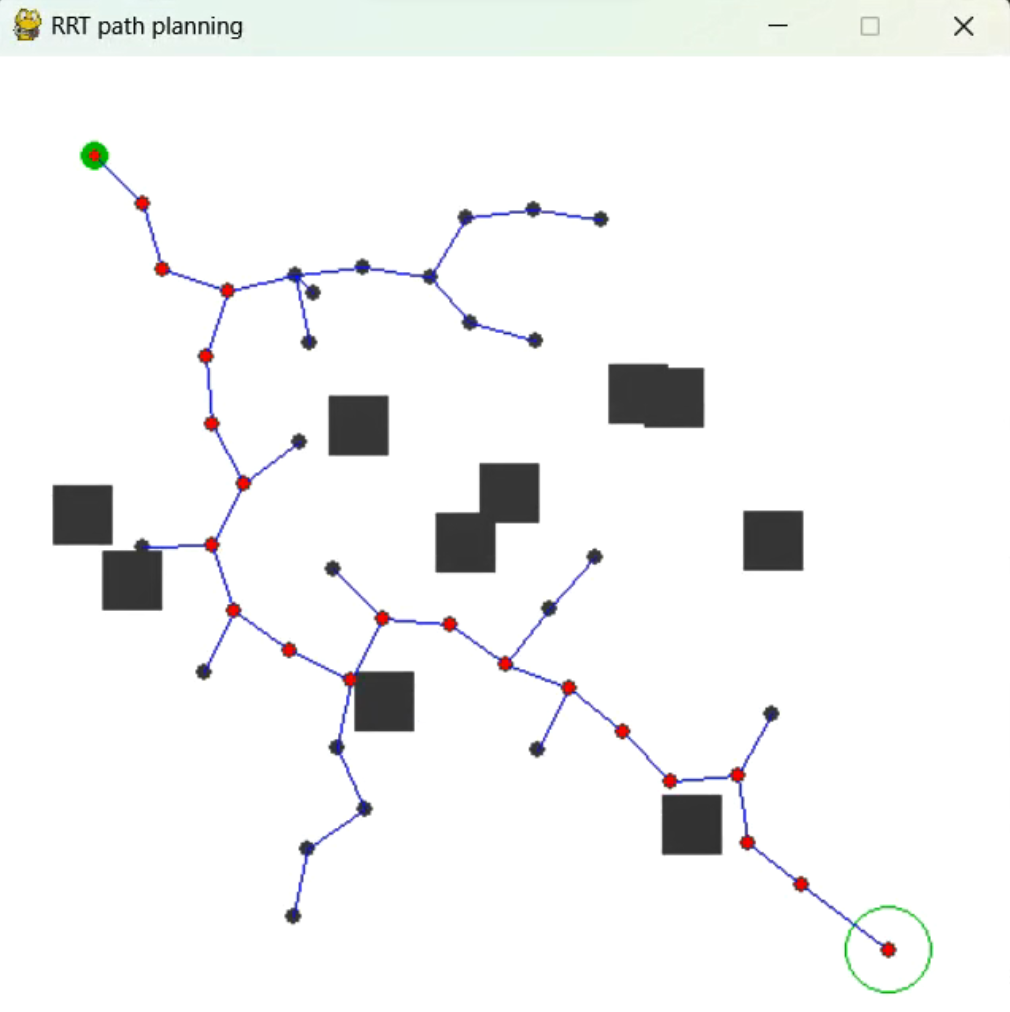
\includegraphics[width=0.7\textwidth]{./images/Chapter2/ConvexResult}	
	\caption[شبیه سازی الگوریتم \lr{RRT}]{شبیه سازی الگوریتم \lr{RRT}}
	\label{نتیجه شبیه‌سازی RRT}
\end{figure}
\noindent
\unskip
\newpage

\subsection{نتیجه تشخیص مانع}
در فصل دوم به بررسی نحوه تشخیص موانع به کمک رنگ‌ها و ابعاد آن‌‌ها پرداخته شد. در زیر برخی از نتایج آن قابل مشاهده است:

\begin{figure}[h]
	\centering
	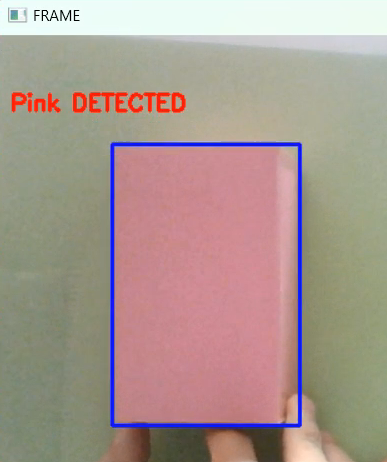
\includegraphics[width=0.6\textwidth]{./images/Chapter2/PinkDetected}	
	\caption[مانع مکعب مستطیل با رنگ صورتی]{مانع مکعب مستطیل با رنگ صورتی}
	\label{PinkDetected}
\end{figure}
\noindent
\unskip

\newpage
\subsection{نتایج پیاده‌سازی عملی}
همان‌طور که در فصل‌های قبل اشاره شد برای پیاده‌سازی عملی ملاحظاتی برای ادغام الگوریتم با ویژگی‌های ربات صورت گرفت و تصویر زیر یکی از نتایج عملی ربات است که با تشخیص مانع آبی‌رنگ و ارتفاع آن تصمیم به عبور از روی این مانع گرفته است.

\begin{figure}[h]
	\centering
	\subfloat[ نمای بالا]{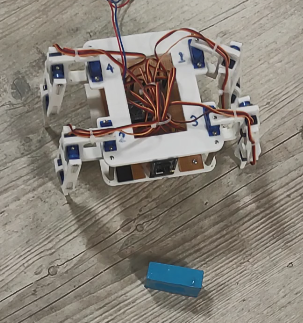
\includegraphics[width=4cm]{./images/Chapter5/BlueBackUpview}}
	\qquad
	\subfloat[ نمای روبرو]{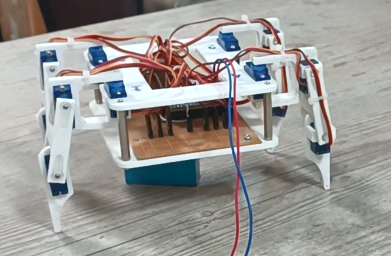
\includegraphics[width=6cm]{./images/Chapter5/BlueUp}}
	\caption{تشخیص رنگ آبی}
	%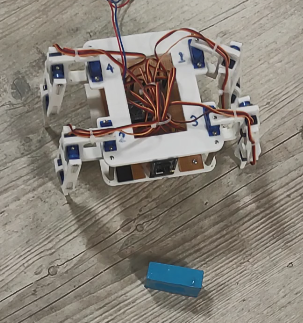
\includegraphics[width=0.4\textwidth]{./images/Chapter5/BlueBackUpview}	
	%\caption[-نمای بالا از ربات تشخیص رنگ آبی]{تشخیص رنگ آبی- نمای بالا از ربات}
	\label{تشخیص رنگ آبی}
\end{figure}
\noindent
\unskip
% \textbf{تشخیص رنگ آبی توسط ربات و عبور از آن به دلیل ارتفاع کوتاه آن:}
\subsection{نتایج مکان‌یابی}
\label{نتایج مکان‌یابی}
همان‌طور که نحوه مکان‌یابی ربات در فصل دوم بررسی گردید، با استفاده از تگ‌‌هایی که اطلاعات فاصله و زاویه دوربین نسبت به آن‌‌ها را برمی‌گردانند و با دانستن موقعیت هر کدام از تگ‌ها به موقعیت ربات در هر لحظه دست می‌یابیم. نتایج حاصل از این مکان‌یابی در شکل زیر آمده است:
\begin{figure}[h]
	\centering
	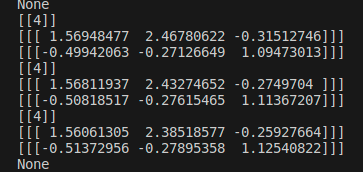
\includegraphics[width=0.6\textwidth]{./images/Chapter5/arucoMatrices}	
	\caption[ زوایا و فواصل از تگ]{زوایا و فواصل از تگ}
	\label{مکان‌یابی}
\end{figure}
\noindent
\unskip

در این شکل دو ماتریس که هر کدام دارای سه المان هستند و یک عدد که بیانگر شماره تگ رویت شده است، قابل‌مشاهده است.  ماتریس اول  بیانگر زاویه تگ با دوربین ربات و ماتریس دوم بیانگر فاصله دوربین و تگ (بر حسب متر) در هر کدام از محور‌های مختصات است.
\newpage
\section{پیشنهادات}
در اين قســمت باتوجه‌به كارهای انجام شــده در اين پژوهش و نتايج حاصــل شــده، پيشــنهاداتی برای كارهای آينده، به شرح زير ارائه مي‌گردد:
\begin{itemize}
	\item
	می‌توان از دوربین‌ باکیفیت بالاتر استفاده کرد تا در شرایط محیطی متفاوت که میزان نور و... در تشخیص رنگ‌ها تأثیرگذار هستند بادقت بیشتری بررسی شوند.
	\item
	استفاده از الگوریتم‌های دیگر مسیریابی و آزمایش عملی بر روی ربات برای دسترسی به روشی بهینه 
	
\end{itemize}